% Figure 4: Dual Collapse Criterion
% Showing convergence of Penrose gravitational threshold and VFD coherence threshold
\documentclass[tikz,border=5pt]{standalone}
\usepackage{tikz}
\usetikzlibrary{calc,decorations.pathmorphing,arrows.meta,shapes.geometric,positioning}

\begin{document}
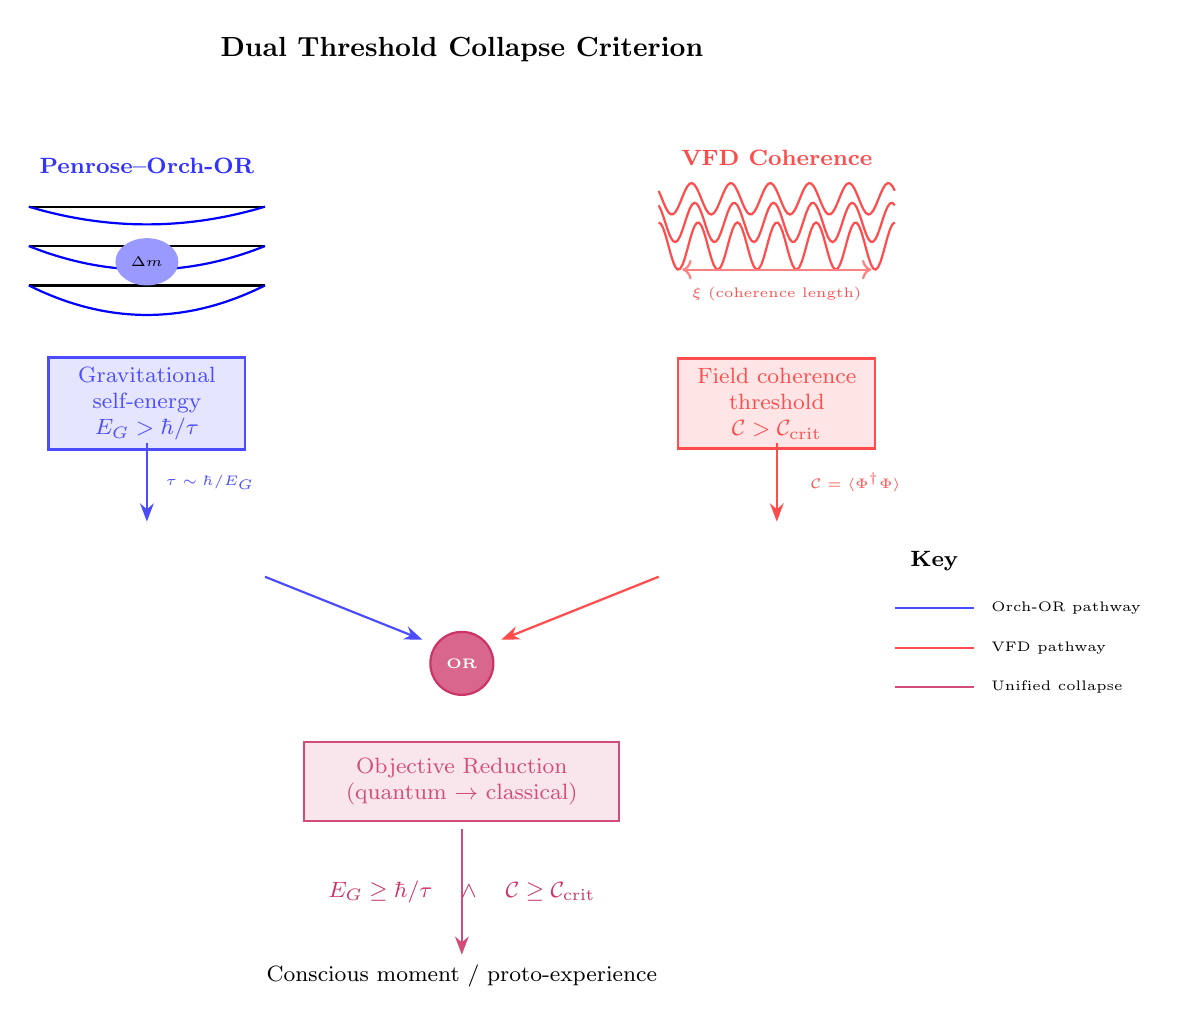
\begin{tikzpicture}[scale=1,
    block/.style={rectangle,draw,thick,minimum width=2.5cm,minimum height=1cm,align=center,font=\footnotesize},
    arrow/.style={->,thick,>=Stealth}
]

% === Title ===
\node[font=\bfseries] at (0,5) {Dual Threshold Collapse Criterion};

% === LEFT PATH: Penrose Gravitational (Orch-OR) ===
\begin{scope}[shift={(-4,0)}]
    % Spacetime curvature visualization
    \draw[thick] (-1.5,3) -- (1.5,3);
    \draw[thick] (-1.5,2.5) -- (1.5,2.5);
    \draw[thick] (-1.5,2) -- (1.5,2);
    % Curved spacetime (mass-induced)
    \draw[thick,blue] (-1.5,3) .. controls (-0.5,2.7) and (0.5,2.7) .. (1.5,3);
    \draw[thick,blue] (-1.5,2.5) .. controls (-0.5,2.1) and (0.5,2.1) .. (1.5,2.5);
    \draw[thick,blue] (-1.5,2) .. controls (-0.5,1.5) and (0.5,1.5) .. (1.5,2);

    % Mass blob
    \fill[blue!40] (0,2.3) ellipse (0.4 and 0.3);
    \node[font=\tiny] at (0,2.3) {$\Delta m$};

    \node[above,font=\footnotesize\bfseries,blue!80] at (0,3.3) {Penrose--Orch-OR};

    % Criterion box
    \node[block,blue!70,fill=blue!10] at (0,0.5) {Gravitational\\self-energy\\$E_G > \hbar/\tau$};

    % Arrow down
    \draw[arrow,blue!70] (0,0) -- (0,-1);

    % Threshold label
    \node[font=\tiny,blue!70] at (0.8,-0.5) {$\tau \sim \hbar/E_G$};
\end{scope}

% === RIGHT PATH: VFD Coherence ===
\begin{scope}[shift={(4,0)}]
    % Coherent wave pattern
    \draw[thick,red!70,domain=-1.5:1.5,samples=100] plot (\x,{2.5+0.3*cos(720*\x)});
    \draw[thick,red!70,domain=-1.5:1.5,samples=100] plot (\x,{2.8+0.25*cos(720*\x+30)});
    \draw[thick,red!70,domain=-1.5:1.5,samples=100] plot (\x,{3.1+0.2*cos(720*\x+60)});

    % Coherence indicator
    \draw[<->,red!50,thick] (-1.2,2.2) -- (1.2,2.2);
    \node[below,font=\tiny,red!70] at (0,2.1) {$\xi$ (coherence length)};

    \node[above,font=\footnotesize\bfseries,red!70] at (0,3.4) {VFD Coherence};

    % Criterion box
    \node[block,red!70,fill=red!10] at (0,0.5) {Field coherence\\threshold\\$\mathcal{C} > \mathcal{C}_{\mathrm{crit}}$};

    % Arrow down
    \draw[arrow,red!70] (0,0) -- (0,-1);

    % Threshold label
    \node[font=\tiny,red!70] at (1,-0.5) {$\mathcal{C} = \langle\Phi^\dagger\Phi\rangle$};
\end{scope}

% === CONVERGENCE ZONE ===
\begin{scope}[shift={(0,-2.5)}]
    % Convergence arrows
    \draw[arrow,blue!70,thick] (-2.5,0.8) -- (-0.5,0);
    \draw[arrow,red!70,thick] (2.5,0.8) -- (0.5,0);

    % Central collapse event
    \fill[purple!60] (0,-0.3) circle (0.4);
    \draw[thick,purple!80] (0,-0.3) circle (0.4);
    \node[white,font=\tiny\bfseries] at (0,-0.3) {OR};

    % Collapse box
    \node[block,purple!70,fill=purple!10,minimum width=4cm] at (0,-1.8) {Objective Reduction\\(quantum $\to$ classical)};

    % Unified condition
    \node[font=\footnotesize,purple!80] at (0,-3.2) {$E_G \geq \hbar/\tau \quad \wedge \quad \mathcal{C} \geq \mathcal{C}_{\mathrm{crit}}$};

    % Output
    \draw[arrow,purple!70] (0,-2.4) -- (0,-4);
    \node[below,font=\footnotesize] at (0,-4) {Conscious moment / proto-experience};
\end{scope}

% === Legend / Key ===
\begin{scope}[shift={(6,-3)}]
    \node[font=\footnotesize\bfseries] at (0,1.5) {Key};
    \draw[blue!70,thick] (-0.5,0.9) -- (0.5,0.9);
    \node[right,font=\tiny] at (0.6,0.9) {Orch-OR pathway};
    \draw[red!70,thick] (-0.5,0.4) -- (0.5,0.4);
    \node[right,font=\tiny] at (0.6,0.4) {VFD pathway};
    \draw[purple!70,thick] (-0.5,-0.1) -- (0.5,-0.1);
    \node[right,font=\tiny] at (0.6,-0.1) {Unified collapse};
\end{scope}

\end{tikzpicture}
\end{document}
